\documentclass[border=3pt]{standalone}
\usepackage[T1]{fontenc}
\usepackage{tikz}
\usetikzlibrary{positioning, arrows.meta, fit, backgrounds, calc, shapes.geometric}

\definecolor{ueblue}{HTML}{1565C0}
\definecolor{gnbgreen}{HTML}{2E7D32}
\definecolor{jamred}{HTML}{C62828}
\definecolor{ricpurple}{HTML}{6A1B9A}
\definecolor{rappamber}{HTML}{E65100}
\definecolor{coregray}{HTML}{37474F}
\definecolor{lightbg}{HTML}{F5F5F5}
\definecolor{ricbg}{HTML}{EDE7F6}
\definecolor{nrtbg}{HTML}{FFF3E0}

\begin{document}
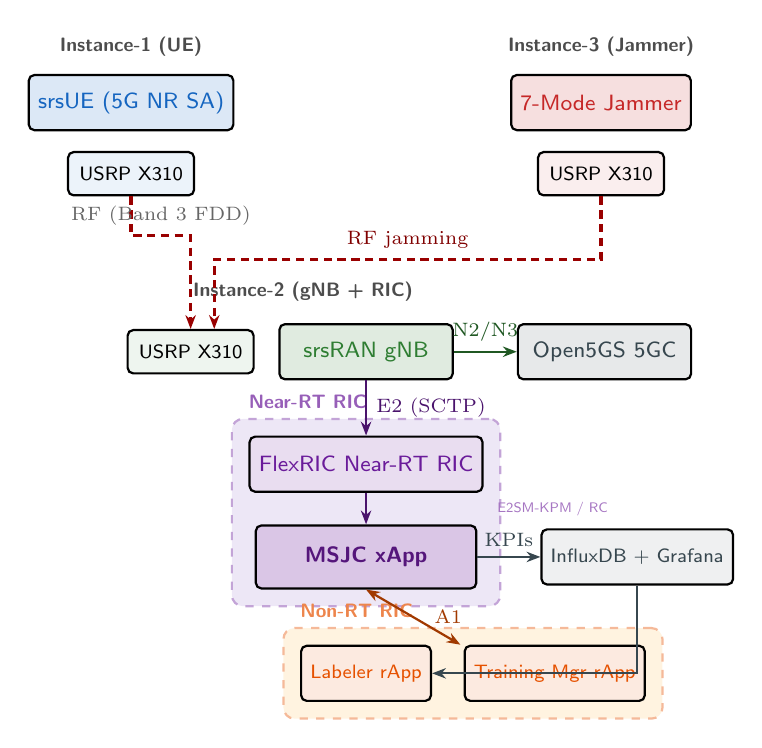
\begin{tikzpicture}[
    node distance=0.6cm and 1.2cm,
    box/.style={draw, rounded corners=2pt, minimum height=0.7cm, minimum width=2.2cm,
                font=\footnotesize\sffamily, thick, fill=white},
    hwbox/.style={draw, rounded corners=2pt, minimum height=0.55cm, minimum width=1.6cm,
                  font=\scriptsize\sffamily, thick, fill=white},
    label/.style={font=\scriptsize\sffamily\bfseries, text=black!70},
    arr/.style={-{Stealth[length=5pt]}, thick},
    darr/.style={{Stealth[length=5pt]}-{Stealth[length=5pt]}, thick},
    rfarr/.style={-{Stealth[length=5pt]}, very thick, red!60!black, densely dashed},
  ]

  % ── Instance-1 (UE) ──
  \node[box, fill=ueblue!15, text=ueblue] (ue) {srsUE (5G NR SA)};
  \node[hwbox, below=0.25cm of ue, fill=ueblue!8] (ue_usrp) {USRP X310};
  \node[label, above=0.1cm of ue] {Instance-1 (UE)};

  % ── Instance-3 (Jammer) ──
  \node[box, fill=jamred!15, text=jamred, right=3.5cm of ue] (jam) {7-Mode Jammer};
  \node[hwbox, below=0.25cm of jam, fill=jamred!8] (jam_usrp) {USRP X310};
  \node[label, above=0.1cm of jam] {Instance-3 (Jammer)};

  % ── Instance-2 (gNB + RIC) ──
  \node[box, fill=gnbgreen!15, text=gnbgreen, below=2.8cm of $(ue)!0.5!(jam)$] (gnb) {srsRAN gNB};
  \node[hwbox, left=0.3cm of gnb, fill=gnbgreen!8] (gnb_usrp) {USRP X310};
  \node[label, above=0.15cm of gnb, xshift=-0.8cm] {Instance-2 (gNB + RIC)};

  % 5GC
  \node[box, fill=coregray!12, text=coregray, right=0.8cm of gnb] (core) {Open5GS 5GC};

  % Near-RT RIC
  \node[box, fill=ricpurple!15, text=ricpurple, below=0.7cm of gnb, minimum width=2.4cm] (ric) {FlexRIC Near-RT RIC};
  \node[box, fill=ricpurple!25, text=ricpurple!80!black, below=0.4cm of ric, minimum width=2.8cm, minimum height=0.8cm]
    (xapp) {\textbf{MSJC xApp}};

  % Observability
  \node[box, fill=coregray!8, text=coregray, right=0.8cm of xapp, minimum width=1.8cm, font=\scriptsize\sffamily]
    (influx) {InfluxDB + Grafana};

  % Non-RT RIC rApps
  \node[box, fill=rappamber!12, text=rappamber, below=0.7cm of xapp, minimum width=1.6cm, font=\scriptsize\sffamily]
    (labeler) {Labeler rApp};
  \node[box, fill=rappamber!12, text=rappamber, right=0.4cm of labeler, minimum width=1.9cm, font=\scriptsize\sffamily]
    (trainer) {Training Mgr rApp};

  % ── Background boxes ──
  \begin{scope}[on background layer]
    \node[draw=ricpurple!40, fill=ricbg, rounded corners=4pt, dashed, thick,
          fit=(ric)(xapp), inner sep=6pt] (ricbox) {};
    \node[draw=rappamber!40, fill=nrtbg, rounded corners=4pt, dashed, thick,
          fit=(labeler)(trainer), inner sep=6pt] (nrtbox) {};
    \node[label, text=ricpurple!70] at (ricbox.north west) [anchor=south west, xshift=3pt] {Near-RT RIC};
    \node[label, text=rappamber!70] at (nrtbox.north west) [anchor=south west, xshift=3pt] {Non-RT RIC};
  \end{scope}

  % ── RF links ──
  \draw[rfarr] (ue_usrp.south) -- ++(0,-0.5) -| node[pos=0.25, above, font=\scriptsize, text=black!60] {RF (Band 3 FDD)} (gnb_usrp.north);
  \draw[rfarr] (jam_usrp.south) -- ++(0,-0.8) -| node[pos=0.25, above, font=\scriptsize, text=red!50!black] {RF jamming} ($(gnb_usrp.north)+(0.3,0)$);

  % ── Protocol links ──
  \draw[arr, gnbgreen!70!black] (gnb.east) -- node[above, font=\scriptsize] {N2/N3} (core.west);
  \draw[arr, ricpurple!70!black] (gnb.south) -- node[right, font=\scriptsize] {E2 (SCTP)} (ric.north);
  \draw[arr, ricpurple!70!black] (ric.south) -- (xapp.north);
  \draw[arr, coregray] (xapp.east) -- node[above, font=\scriptsize] {KPIs} (influx.west);
  \draw[darr, rappamber!70!black] (xapp.south) -- node[right, font=\scriptsize, xshift=4pt] {A1} ($(labeler.north)!0.5!(trainer.north)$);
  \draw[arr, coregray] (influx.south) |- (labeler.east);

  % ── E2SM labels ──
  \node[font=\tiny\sffamily, text=ricpurple!60, right=0.05cm of ric.south east, anchor=north west] {E2SM-KPM / RC};

\end{tikzpicture}
\end{document}
